
\section{Angle dependent measurements}
    \label{Sec:ResD:AngleDependentMeasurements}

\subsection{Determining experimental parameters}

Preliminary measurements showed very strong dHvA oscillations which begin at relatively low field.  An example of the raw data can be seen in figure~\ref{Fig:ResD:RawOscillations}. Since it is not clear from the raw torque data where the oscillations begin, Fourier transforms were taken with small (\unit[1]{T}) field intervals --- the interval where a clear signal is present marks the onset of oscillations. A FFT of the data for the ranges \unit[4-5]{T}, \unit[5-6]{T} and \unit[6-7]{T} are shown in the insets of the figure. The range \unit[6-7]{T} clearly shows the electron peaks at around \unit[1500]{T} and \unit[2450]{T}, with the higher frequency peak disappearing in the \unit[5-6]{T} range and both peaks disappearing in the \unit[4-5]{T} range. Further refinement suggests the onset of appreciable oscillations is around \unit[5.6]{T} for the strongest electron peak. The field was ramped between \unit[6]{T} and the safe maximum of \unit[18]{T} for the vast majority of measurements bar some sweeps where the magnet was ramped to or from \unit[0]{T} following or preceding shut-down of the magnet.
%%
\begin{figure}[htbp]
    \begin{center}
        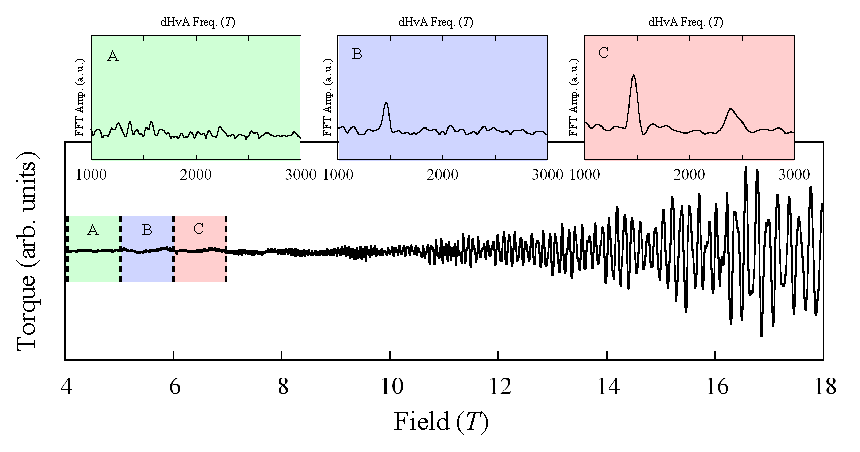
\includegraphics[scale=0.7]{Chapter-dHvABaFe2P2/Figures/AngleDepMeasurements/RawOscillations/RawOscillations}
        \caption{An example of the torque data taken with field aligned at \unit[26]{\degree} on the reverse side of the $[001]$ to $[100]$ angle sweep detailed later. Insets show a FFTs of the data between \unit[4-5]{T}, \unit[5-6]{T} and \unit[6-7]{T} respectively. These intervals are marked on the main plot as A, B and C.}
        \label{Fig:ResD:RawOscillations}
    \end{center}
\end{figure}

 Figure~\ref{Fig:ResD:ComparisonSweepRates} shows some example Fourier transforms of data taken at various field sweep rates and plotted with the frequencies shifted arbitrarily for ease of comparison. The difference in amplitude between the sweeps at \unit[0.05]{T/min.} and \unit[0.1]{T/min.} is less than \unit[1]{\%} whereas the difference when sweeping at \unit[0.2]{T/min.} is nearly \unit[5]{\%}. Unless otherwise stated, subsequent sweeps were performed at \unit[0.1]{T/min.}.
%%
\begin{figure}[htbp]
    \begin{center}
        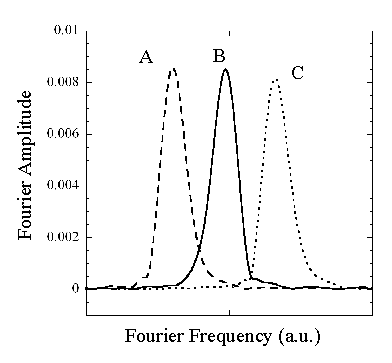
\includegraphics[scale=0.7]{Chapter-dHvABaFe2P2/Figures/AngleDepMeasurements/SweepRateComparison/SweepRateComparison}
        \caption{FFTs showing the peak from the smaller branch of band $3$ taken at, A: \unit[0.05]{T/min.}, B: \unit[0.1]{T/min.} and C: \unit[0.2]{T/min.}. The peaks are arbitrarily shifted in frequency for ease of comparison. Measurements taken with $H$ at \unit[10]{\degree} from $[001]$ in the $[110]$ direction.}
        \label{Fig:ResD:ComparisonSweepRates}
    \end{center}
\end{figure}

In order to make a reasonable determination of the Fermi surface of a material, an appropriate number of angle sweeps need to be made to adequately constrain the shape of the Fermi surface. Since \BaFeP is a tetragonal system, any sweep from the azimuthal direction $[001]$ down the polar plane effectively expands to four due to the fourfold symmetry. Measurements were taken at one degree intervals from $H\parallel[001]$ down to $H\parallel[100]$ and from $H\parallel[001]$ down to $H\parallel[110]$ which, in this system, effectively amount to eight sweeps.

The magnetic field was alternatively ramped up and then down meaning subsequent measurements were generally performed with the magnetic field ramping in opposite directions. Although in theory this should not affect the results in any way, subsequent FFT peaks appeared to alternately be shifted by up to $\sim\pm$\unit[21]{T} with the magnitude of the shifts being roughly proportional to frequency. Assuming that the shifts were an artefact of the measurements, a linear correction determined by visual inspection was applied of $F_{\textrm{corr.}} = 3 + \frac{10}{8000} F_{\textrm{meas.}}$ for the sweep in the $[100]$ direction and $F_{\textrm{corr.}} = 0 + \frac{21}{8000}  F_{\textrm{meas.}}$ and  $F_{\textrm{corr.}} = 0 + \frac{18}{8000} F_{\textrm{meas.}}$ for the two sets of measurements performed to complete the sweep in the $[110]$ direction.

%%
\begin{figure}[htbp]
    \begin{center}
        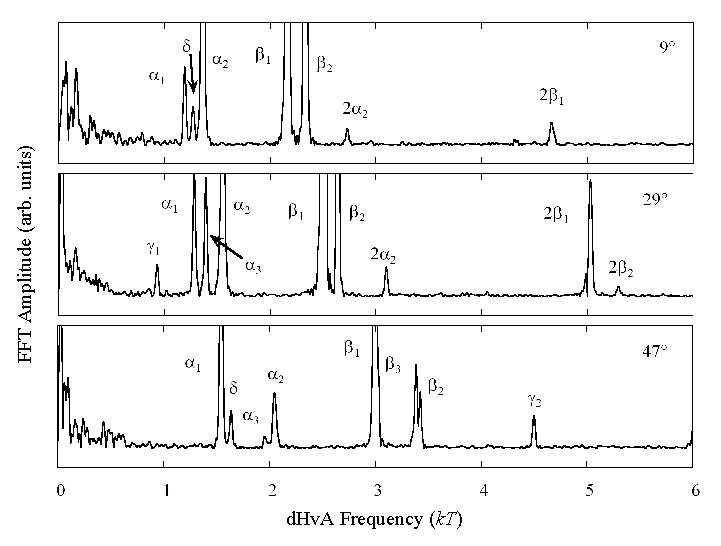
\includegraphics[scale=0.7]{Chapter-dHvABaFe2P2/Figures/AngleDepMeasurements/FFTExamples/FFTExamples}
        \caption{FFT after a second order polynomial background was subtracted at various labelled angles between $[001]$ and $[110]$. The labels for peak identification are explained in the next section.}
        \label{Fig:ResD:FFTExamples}
    \end{center}
\end{figure}
%%
Figure~\ref{Fig:ResD:FFTExamples} shows three example FFTs which show peaks from all the principal bands identified the next section. They also show first and second harmonics\footnote{Third harmonics were also identified in other FFTs, these are shown in figure~\ref{Fig:ResD:AngleSweepMeasured}.}. The low frequency region in figure~\ref{Fig:ResD:FFTExamples} shows noise from the cantilever, but according to DFT fits performed in the next section, this region also likely contains signal from the minimum of band $1$. Given that the signal from electron bands is generally small due to high scattering rate, we were not able to extract a convincing Fourier peak.

Figure~\ref{Fig:ResD:AngleSweepMeasured} shows the set of peak data after having the angle determined as described in section~\ref{Sec:2:AngleCorrection}. The points marked in grey are the harmonics which were identified by overlaying the measured data on itself after doubling and tripling of the frequency. Signal can be observed up to relatively high angles for the torque technique ($R_T \propto \sin{\theta}$) with peak observed almost up to $80\degree$  in the $[110]$ direction which, along with the observation of third harmonics, and the onset of oscillations in relatively low field is further testament to the quality of the crystal.
%%
\begin{figure}[htbp]
    \begin{center}
        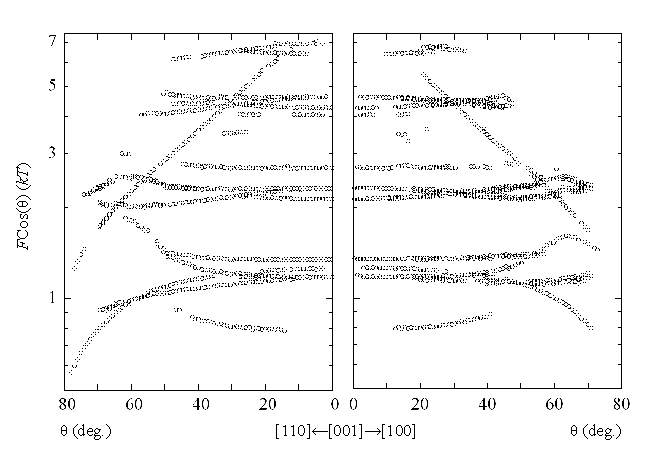
\includegraphics[scale=0.9]{Chapter-dHvABaFe2P2/Figures/AngleDepMeasurements/AngleSweepMeasured/AngleSweepMeasured}
        \caption{Peaks identified by varying the field range, window type and background polynomial. Left panel shows data taken with the field parallel to $[001]$ down to $[110]$, the right panels shows $[001]$ to $[100]$. Points marked in grey are harmonics.}
        \label{Fig:ResD:AngleSweepMeasured}
    \end{center}
\end{figure}
%%
Figure~\ref{Fig:ResD:SubstitutionComparison} shows the measured rotation data which has been matched up to corresponding orbits in the DFT calculations (see next section). Superimposed is the data from the $x=0.63$ data in the \BaFePAs series multiplied by amounts commensurate to the expected shifts in the Shishido paper\cite{Shishido2010}. We can see that while the size of the areas changes between the two values, the overall shape of the $x=0.63$ data matches reasonably well with the data for $x=1$ for bands 2, 3 and 4 at least. Assuming that nothing exotic happens in the intermediary, we can extrapolate the shape of these Fermi surfaces across the range by applying the known electron Fermi surface areas and the compensation condition. This is explored further in the next section.
%%
\begin{figure}
    \begin{center}
        \includegraphics[scale=0.9]{Chapter-dHvABaFe2P2/Figures/AngleDepMeasurements/SubstitutionComparison/SubstitutionComparison}
        \caption{dHvA data taken with the field rotating from $[001]\rightarrow[100]$. Overlaid in black squares is data from BaFe$_2$As$_{0.37}$P$_{0.63}$\cite{Analytis2010c} with the $\alpha$ and $\gamma$ frequencies multiplied by $1.33$ and $\beta$ frequencies multiplied by $1.19$ commensurate with known shifts from literature. Data is colour coded according to the bands identified from DFT calculations detailed later.}
        \label{Fig:ResD:SubstitutionComparison}
    \end{center}
\end{figure}
%%

\clearpage

\subsubsection{Rigidly shifting the calculated DFT energies}
    \label{Sec:ResD:DFTShifts}

Figure~\ref{Fig:ResD:AngleSweepMeasuredUnshifted} shows the DFT calculations performed using the augmented plane wave method plus local orbits method method as implemented in the WIEN2k package\cite{Blaha2001}. The unit cell used was that measured by Rotter et al. which are listed in table~\ref{Tab:ResD:LatticeParams}. The calculations were processed into rotation plots using the MATLAB code originally written by Dr. Ed Yelland. Results are shown superimposed over the measured data. By factoring the frequency with $\cos{\theta}$ it becomes clearer which of the orbits is a maximal extrema and which is a minimal extrema. Using this knowledge as well as clues from the Fourier amplitude of the measured data, it was possible to separate out individual bands which have been colour coded and labelled --- according to literature convention --- as specified in table~\ref{Tab:ResD:BandNaming}. Minimal extrema are sub-labelled $1$, maxima are sub-labelled $2$.
%%
\begin{table}
    \begin{center}
        \caption{A summary of the Fermi surface labelling used.}
        \begin{tabular}[htbp]{llll}
\toprule
Band Num.  & Label & Colour    & Type \\
\midrule
1   & $\delta$  & Orange    & hole \\
2   & $\gamma$  & Red   & hole \\
3   & $\beta$   & Blue  & electron \\
4   & $\alpha$  & Green & electron \\
\bottomrule
        \label{Tab:ResD:BandNaming}
        \end{tabular}
    \end{center}
\end{table}
%%
As with previous DFT calculations in the \BaFePAs series, the calculated values are consistently higher than the measured values. The exception in this case is $\gamma_2$ which is not much different from the calculated values.
%%
\begin{figure}
    \begin{center}
        \includegraphics[scale=0.7]{Chapter-dHvABaFe2P2/Figures/AngleDepMeasurements/AngleSweepMeasuredUnshifted/AngleSweepMeasuredUnshifted}
        \caption{dHvA frequencies multiplied by $\cos(\theta)$. Solid lines are DFT calculations, open circles are measured data. $H$ field directed along $[001]\rightarrow[100]$.}
        \label{Fig:ResD:AngleSweepMeasuredUnshifted}
    \end{center}
\end{figure}

For the $[110]$ direction it became apparent from the fact that the DFT and the measured curves were qualitatively different that the field was not perfectly aligned with the $[110]$ axis of the sample. By assuming that the measurements were taken from the $c$-axis direction down to a vector rotated \unit[10]{\degree} within the $ab$-plane from the $[110]$ direction, the DFT data matches much better. A \unit[10]{\degree} misalignment is within the estimated alignment error for the microscope images. The data will continue to be labelled as in the $[110]$ plane however for convenience.

As is shown in figure~\ref{Fig:ResD:AngleSweepMeasuredUnshifted}, the rotation plots from the DFT calculations match up qualitatively with the data but do not match up quantitatively -- the electron bands overestimating the size of the measured extremal orbits. 

\begin{figure}[htbp]
    \begin{center}
        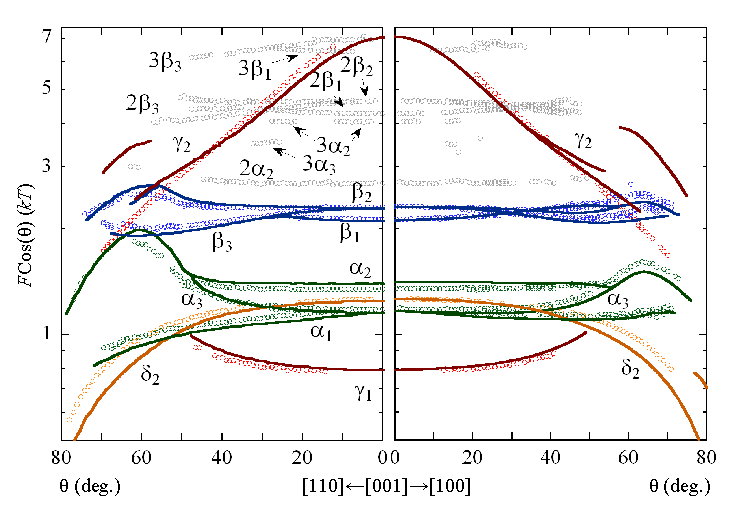
\includegraphics[scale=0.9]{Chapter-dHvABaFe2P2/Figures/AngleDepMeasurements/AngleSweepRigidShift/AngleSweepRigidShift}
        \caption{dHvA frequencies multiplied by $\cos(\theta)$. Solid lines are rigidly shifted DFT calculations, open circles are measured data. $H$ field directed along $[001]$ towards (a) $[001]\rightarrow[100]$ and (b) $[001]\rightarrow[110]$.}
        \label{Fig:ResD:AngleSweepRigidShift}
    \end{center}
\end{figure}

In order to obtain the correct shape of Fermi surface, the DFT calculations need to be tweaked. One technique is to apply small band-specific rigid energy shifts, which, in most cases is enough to bring the DFT in line with the experimental data. figure~\ref{Fig:ResD:AngleSweepRigidShift} shows the rotation plots which rotate towards both the 100 and 110 directions along with appropriately shifted calculations. Table~\ref{Tab:ResD:EnergyShifts} lists those energy shifts.
\begin{table}
    \begin{center}
        \caption{Rigid energy shifts required to match the DFT calculations with the measured data.}
        \begin{tabular}[htbp]{llr}
\toprule
Band    & \multicolumn{2}{l}{Energy Shift (\unit{Ry})} \\
\midrule
1       &       & -0.0083      \\
2       & Wide  & 0.0          \\
        & Narrow & -0.0038     \\
3       &       & 0.0043       \\
4       &       & 0.0050        \\
\bottomrule
        \label{Tab:ResD:EnergyShifts}
        \end{tabular}
    \end{center}
\end{table}

Band $2$ in this case has two separate shifts specified in two different regions of the Brillouin zone. The rotation plot for the wider orbit located at the edge of the Brillouin zone was calculated with no energy shift and the narrow part of the Fermi surface around the $\Gamma$ point was calculated with a shift of $0.0038\unit{Ry}$. This provides a reasonable match for the rotation plot where we can apply the shift to the two regions discretely, however is proves problematic when we wish to study intermediate areas since it is not clear how the Fermi surface varies between the two regions. A technique for applying appropriate energy shifts throughout the Brillouin zone is explored in the next section.

In the first place, these shifts were applied as they conveniently and effectively corrected the Fermi surface energies, however the question arises as to whether there is any physical significance to be attached to them. The technique of rigid energy corrections has been applied to previous measurements on LaFePO\cite{Carrington2009} and SrFe$_2$P$_2$\cite{Analytis2009} both of which are highly two dimensional systems that exhibit relatively strong nesting characteristics. This is in contrast with measurements on CaFe$_2$P$_2$\cite{Coldea2009} which has a highly three dimensional Fermi surface and no nesting vector. Furthermore the bulbous area of the three dimensional hole surface in \BaFeP which does not nest requires no shifting of the Fermi surface to match DFT calculations, whereas the nested neck portion does require a shift. This correlation between nesting and shifts in calculated energy make the spin-density-wave fluctuations that are associated with the nesting phenomena an obvious candidate for the cause of the discrepancy between DFT calculation and experiment.


\subsubsection{Shifting the DFT calculations proportional to orbital character}
\label{Sec:ShiftingDFTPropToOrbitalCharacter}

Figure~\ref{Fig:ResD:Band2DCharacter} shows the partial orbital character for for each of the bands along the path of Fermi surface contour in a $[110]$ slice through the \BaFeP \ac{BZ} as a function of $k_z$. The top row of plots show the character broke down by atomic contribution, the middle row is broken down by the $s$, $p$, $d$ and $f$ contributions to the iron contribution and the bottom row breaks down the iron $d$ character into its sub orbitals.
% Band characters for the other bands presented in a similar way can be found in Appendix~\ref{Appendix:BandCharacter110Slices}.%%
% \begin{figure}[htbp]
%     \begin{center}
%         \includegraphics[scale=0.8]{Chapter-dHvABaFe2P2/Figures/AngleDepMeasurements/BandCharacterPlot/Band2_110Slice_BandCharacter}
%         \caption{Partial $d$-orbital character of the hole band $2$ across slices in the 110 direction. Solid lines show the Fermi surface in the plane.}
%         \label{Fig:ResD:Band2DCharacter}
%     \end{center}
% \end{figure}
%%
\begin{figure}[htbp]
    \begin{center}
        \includegraphics[scale=0.95]{Chapter-dHvABaFe2P2/Figures/AngleDepMeasurements/BandCharacterVsKz/AllBandCharacterVsKz}
        \caption{Partial characters along the Fermi surface contour in the 110 slice (shown in insets) vs. \kz. Top row is the chaacrter broken down by each atom, middle row is the iron contribution broken down into the $l$ orbital contributions, the bottom row is the iron $d$ orbital contributions broken down into its suborbitals.}
        \label{Fig:ResD:Band2DCharacterVsKz}
    \end{center}
\end{figure}
We can see the vast majority of Fermi surface chaarcter is due to the iron atomic contributions with some phosphor for bands 2 and 3 which corresponds well to the notion of FeP conducting planes\TODO{Why does the total not sum to 1?}. For all the bands, the overwhelming majority of the contribution from the iron atoms is from the $d$ orbitals and so other contributions are ignored.

Band $2$ has very little basel-plane \Dxy and \DxTwoyTwo character close to the Fermi level but shows a significant amount of \DzTwo character at the wide region of the Fermi surface and \DxzDyz character at the narrow region. Evidently, energy shifts could be applied which are scaled to either the \DzTwo and \DxzDyz orbital character in order that we obtain a smooth energy shift transition between the narrow and wide regions discussed previously. 

Energy shifts were applied across the full three dimensional Brillouin zone for band $2$ using the following two scalings which were determined by trial and error fitting of the data,
%%
\begin{align*}
\textrm{\DzTwo:}\quad \Delta\epsilon &= 0.002 - 0.0052 \left(1 - \frac{\epsilon - 0.033}{0.2205 - 0.033}\right) \\
\textrm{\DxzDyz:}\quad \Delta\epsilon &= 0.002 - 0.0052 \left(\frac{\epsilon - 0.0946}{0.3135 - 0.0946}\right)
\end{align*}
%%
Note that these scalings ensure that the energy shift applied varies between \unit[-32]{mRy} and \unit[2]{mRy} which are slightly different to the values applied when rigidly shifting the band. This is due to the fact that the Fermi surface area measured in the narrow region is affected more and more by the size of the Fermi surface in the wide region (and vice-versa) as the azimuthal angle gets higher. The calculated area deviates from the measured area which results in the crossing of the calculated rotation plot with the measured rotation plot shown in the first panel of figure~\ref{Fig:ResD:Band2DCharacterRigidComparison}. So when the rigid shifts were being determined, values were chosen which best lines up along the full length of the curve -- one which will be slightly lower than if we were to match the plots exactly at $\theta=0^\circ$.

\begin{figure}[htbp]
    \begin{center}
        \includegraphics[scale=0.8]{Chapter-dHvABaFe2P2/Figures/AngleDepMeasurements/BandCharacterRotPlot/Band2_110_RotPlot_Comparison}
        \caption{dHvA frequencies for band 2 multiplied by the cosine of the angle of the $H$ field. $H$ field directed along $[001]\rightarrow[110]$. Open circles are measured data, solid lines represent (a) rigidly shifted DFT calculations, (b) DFT calculations shifted proportional to \DzTwo orbital character, (c) DFT calculations shifted proportional to \DxzDyz orbital character.}
        \label{Fig:ResD:Band2DCharacterRigidComparison}
    \end{center}
\end{figure}

The second and third panels of figure~\ref{Fig:ResD:Band2DCharacterRigidComparison} show the rotation plots calculated with the energy shifts applied proportional to \DzTwo and \DxzDyz orbital character respectively. We observe a much better alignment of the measured and calculated data for all angles. Figure~\ref{Fig:ResD:BandCharacterFSShiftComparison} shows the Fermi surfaces before and after shifting using the rigid energy shifts for bands $1$, $3$ and $4$ and using shifts scaled to \DzTwo orbital character for band $2$. Figure~\ref{Fig:ResD:FullBandCharacterFermiSurface} shows the assembled unit cell for \BaFeP from the corrected DFT calculations and figure~\ref{Fig:ResD:ShiftedBandStructure} shows the shifted band structure for the bands that cross the Fermi level.
%%
\begin{figure}[htbp]
    \begin{center}
        \includegraphics[scale=0.8]{Chapter-dHvABaFe2P2/Figures/AngleDepMeasurements/BandCharacterFermiSurface/BandCharacterFermiSurfaceShiftComparison}
        \caption{Comparison of Fermi surfaces according to DFT calculations both before and after shift corrections are applied. Rigid shifts are applied to bands 1, 3, 4 and shifts proportional to \DzTwo character are applied to band 2.}
        \label{Fig:ResD:BandCharacterFSShiftComparison}
    \end{center}
\end{figure}
%%
\begin{figure}[htbp]
    \begin{center}
        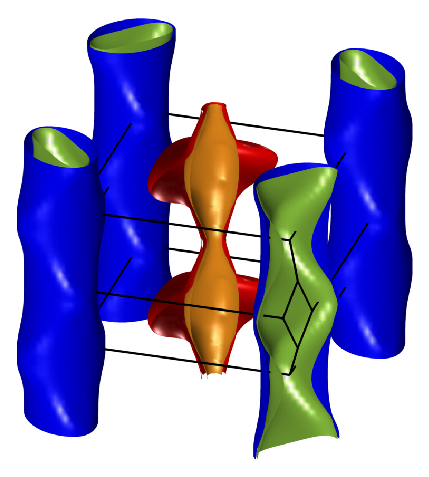
\includegraphics[scale=0.7]{Chapter-dHvABaFe2P2/Figures/AngleDepMeasurements/BandCharacterFermiSurface/FullBandCharacterFermiSurface}
        \caption{Fully assembled Fermi surface in the first Brillouin of \BaFeP as determined by DFT calculations corrected by either rigid energy shifts (bands 1, 3, 4) or shifts proportional to \DzTwo character (band 2)}
        \label{Fig:ResD:FullBandCharacterFermiSurface}
    \end{center}
\end{figure}
%%

The final corrections show the DFT calculations being adjusted in size only for the electron and inner hole surfaces with overall shrinking of volume, the outer hole surface is adjusted in shape as well. Volume calculations as a percentage of the Brillouin zone are given for each of the Fermi surfaces before and after shifting in table~\ref{Table:ResD:FermiSurfaceVolumes},
\begin{table}
    \begin{center}
           \caption{Volumes of the shifted and unshifted Fermi surfaces as a percentage of \ac{BZ} volume.}
        \begin{tabular}[htbp]{lrrr}
\toprule
Band    & Unshifted    & Shifted \DzTwo    & Shifted \DxzDyz \\
\midrule
1  & 5.54\%    & 2.28\%    & 2.28\%    \\
2  & 10.37\%   & 9.74\%    & 9.64\%    \\
3  & (-)9.58\% & (-)7.89\% & (-)7.89\% \\
4  & (-)6.39\% & (-)4.49\% & (-)4.49\% \\
\midrule
Total & -0.065\%    & -0.352\%  & -0.450\%  \\
\bottomrule
        \label{Table:ResD:FermiSurfaceVolumes}
        \end{tabular}
    \end{center}
\end{table}
The volumes compensate better before the shifts by a small amount (\unit[$\sim 0.4$]{\%}) with the shifts proprtional to \DxzDyz being slightly closer to the unshifted volume.

An interesting condition can be seen from figure~\ref{Fig:ResD:ZSlices} where we observe cross sections of the final corrected Fermi surfaces showing the basel-plane at the bottom of the unit cell ($\kz=0$), quarter of the way up, ($\kz=0.25$) and halfway up ($\kz=0.5$). The inner hole surface at $\kz=0.5$ directly matches the size and shape of the inner electron surface at $\kz=0.25$. Moreover both surface share similar predominant \DxzDyz orbital character. Both surfaces have different \kz dispersions which mean nesting along the vector of $q=(\pi, \pi, \pi/2)$ is only partial thus providing the right conditions necessary for possible pair forming spin-density-wave fluctuations. \TODO{Does non-z orbital character preclude nesting with a z component?}
\begin{figure}[htbp]
    \begin{center}
        \includegraphics[scale=0.9]{Chapter-dHvABaFe2P2/Figures/AngleDepMeasurements/ZSlices/ZSlices}
        \caption{Cross sections of the corrected Fermi surface in the $ab$ plane (panels 1, 2 and 3) and in the $[110]$ plane (panel 4). Slices are coloured according to the predominant orbital character of the surface.}
        \label{Fig:ResD:ZSlices}
    \end{center}
\end{figure}
This brings us on to the question of how well nested the Fermi surfaces are. To answer we turn to the calculations of the Lindhard susceptibility.

\clearpage

